\documentclass[10pt]{beamer}

\usepackage[utf8]{inputenc}
\usepackage{pgfpages}
\usepackage{dirtree}
\setbeamertemplate{note page}[plain]
\AtEndNote{\vfill \begin{center} mm:hh \end{center}}
\newcommand{\notedir}[1] {
  \note{\dirtree{#1}}}
\def \ion {$^{\circ}$ }
\usepackage{tcolorbox}
\usepackage{tikz}
\usetikzlibrary{intersections,calc}
\usepackage{amsmath}
\usepackage{graphicx}


\def \heart {\textcolor{blue}{$\heartsuit$} }
\def \C {$\mathcal{C}$}

\tcbset{%
	basic/.style={colframe=black,
		      colback=white,
		      top= 0mm,
		      bottom = 2mm,
		      boxsep=0mm
		      }
                    }

                     \def\enonce{ \frametitle{Q1 Septembre 2015.}
	  On considère deux cercles $\mathcal{C}$ et $\mathcal{C'}$ se coupant en deux points distincts
	  $A$ et $B$. On note $P$ le point diamétralement opposé à $A$ sur $\mathcal{C}$, et $P'$ le
	  point diamétralement opposé à $A$ sur $\mathcal{C'}$ . \\
	  Démontrer que les points $P$ , $B$ et $P'$ sont alignés.
  }
  \def\hypotheses{ \underline{Hypothèses} 
		      \begin{enumerate}
		      \item $[AP]$ diamètre de $\mathcal{C}$ \\
			    $[AP']$ diamètre de  $\mathcal{C'}$,
		      \item $[AB]$ corde de $\mathcal{C}$ et $\mathcal{C'}$.			    
		      \end{enumerate}
}
  \def\these{\underline{Thèse} \\
		      \smallskip
		      $P,B$ et $P'$ alignés.
}

    
\begin{document}  
    \beamertemplatenavigationsymbolsempty
    
    \frame{%enoncé ex1
	  
	 \enonce
	  
	  \vfill
	  
	  \pause
	  % hypothèses et thèse
	  \begin{tcolorbox}[basic] 
	      \begin{columns}[t]
		 
		 \column{.5\textwidth}\centering
		      
		    \hypotheses

		  
		  \column{.5\textwidth}\centering
		      
		      \these
		
	      \end{columns}
	  \end{tcolorbox}
    \notedir{%
    .1 Énoncé.
    .2 Choix : Géométrie synthétique.
    .3 Présence de $\Delta$ et traduction analytique difficile..
    .4 Hypothèses (non visibles sur le dessin)..
    .4 Thèse..
    .4 Grand dessin.. 
    }
    }
    \frame{% résolution ex1

	  \begin{columns}[t]
		\column{.5\textwidth}\centering 
		

			\underline{Dessin}\\
			
				  \begin{figure}[h]
				  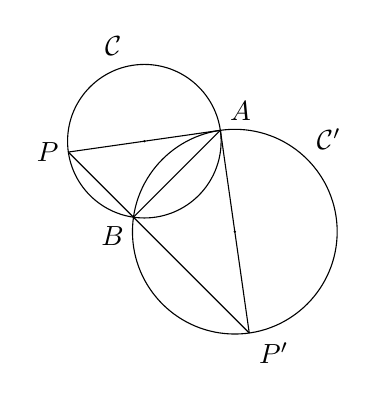
\begin{tikzpicture}[scale=0.65]
					%\draw[help lines] (-3,-3) grid (3,3); 					
					%CERCLE C
					\coordinate (O) at (0,0);
					\fill (O) circle (0.025);
					\draw[name path=cercle] (O) circle (1.5cm);
					\coordinate[label=above left:$\mathcal{C}$] () at (100:1.5);
					%CERCLE C'
					\coordinate (O') at (-45:2.5);
					\fill (O') circle (0.025);
					\draw[name path=cercle'] (O') circle (2cm);
					\path (O') -- +(45:2) coordinate[label=above right:$\mathcal{C'}$] ();

					
					%A et B
					\path [name intersections={of=cercle and cercle',by=intersection}];
					\coordinate[label=above right:$A$] (A) at (intersection-1);
					\coordinate[label=below left:$B$] (B) at (intersection-2);
					\draw (A) -- (O) -- +($(O)-(A)$) coordinate[label=left:$P$](P);
					\draw (A) -- (O') -- +($(O')-(A)$) coordinate[label=below right:$P'$](P');
					\draw (P) -- (P');
					\draw (A) -- (B);
					
				  \end{tikzpicture}
				  \end{figure}
			
				  \begin{tcolorbox}[basic] 
				      
				    \smallskip
				    \hypotheses
							      
				    \these
				    \end{tcolorbox}
		
		
		\column{.5\textwidth}\centering
		
		\underline{Résolution}\\ \flushleft
		
		\heart Un triangle inscrit dans un demi-cercle est rectangle.
		
		$$\begin{cases}
		       \Delta APB \text{ rectangle en } B, \\
		       \Delta AP'B \text{ rectangle en } B.
                     \end{cases}\hspace{-4mm}\rightarrow \widehat{PBP'}=\pi.$$

                     $P$ et $P'$ sont sur une droite $\bot$ à AB passant par $B$.
                     
                     \bigskip
                     
		$P,B$ et $P'$ alignés.  \hfill $\qed$

   
	   \end{columns}
	 \notedir{%
	   .1 Prouver la thèse.
	   .2 Élément de théorie.
	   .3 Triangle inscrit dans demi-cercle..
	   .4 Implique des mesures d'angles..
	   .4 $PBP'$ sont alignés si $\widehat{PBP'}=180^{\circ}$..
	   .2 Résolution.
	   .3 Théorème des triangles inscrits dans demi-cercle..
	   .3 Application à $ABP$ et $ABP'$..
	   .4 $\widehat{ABP}=90^{\circ}$ et $\widehat{ABP'}=90^{\circ}$..
	   .5 $\widehat{PBP'}=180^{\circ} \rightarrow PBP'$ alignés..
	   }   
        }

     \frame{ 
	  \enonce

	  \vfill\center
	  \underline{Résumé}\\ \flushleft
          \begin{itemize}
          \item Montrer que $A,B,C$ sont alignés = montrer que $\widehat{ABC}=\pi$ ?
            \item  Un triangle inscrit dans un demi-cercle est rectangle.
          \end{itemize}
    }
  
\end{document}

%%% Local Variables:
%%% mode: latex
%%% TeX-master: t
%%% End:
